\section{Segmentando el resto del núcleo}

En un primer momento se optó por aplicar un enfoque incremental en lo que respecta a la inserción de los registros de etapa. No obstante, este enfoque se aplicó tan solo en la integración del primer registro de etapa para separar la fase de \textit{fetch} del resto del pipeline. Esto fue así puesto que, de haber seguido integrando registros de etapa uno a uno, verificando el funcionamiento del núcleo con dos, tres y cuatro registros, el proceso de desarrollo se hubiera dilatado en el tiempo más allá de lo deseado inicialmente. Esta aproximación habría requerido resolver de forma independiente, tras la incorporación de cada nuevo registro de etapa a partir del situado entre las fases de \textit{fetch} y decodificación, los problemas derivados de las dependencias de datos y de control entre las instrucciones presentes en el pipeline.

Es por ello por lo que se consideró que resultaría más eficiente integrar los registros de segmentación siguientes al de \textit{fetch}-decodificación a la vez, desarrollando una única solución al problema generado por las dependencias de datos y de control.

Esta solución se ha materializado en el código del módulo \textit{HazardUnit}, cuyo cometido es observar el estado de la arquitectura a cada ciclo para identificar y resolver las dependencias de datos o de control que pudieran originarse durante la ejecución de los programas. A continuación se detalla el método empleado en la resolución de los riesgos de datos del tipo RAW y de control, así como las señales de la \textit{hazard unit} involucradas en el proceso de detección y mitigación del riesgo.

%%%%%%%%%%%%%%%%%%%%%%%%%%%%%%% Resolución de riesgos de datos (RAW) %%%%%%%%%%%%%%%%%%%%%%%%%%%%%%%
\subsection{Resolución de riesgos de datos (RAW)}

En el caso de una arquitectura segmentada en cinco fases, un riesgo de datos del tipo RAW se da cuando en un programa existe una pareja de instrucciones consecutivas para las cuales se cumple que, la segunda de ellas, posee como registro origen en alguno de sus operandos el registro de destino de la primera, pudiendo encontrarse separadas una distancia de 1 o 2 ciclos. Esta casuística queda ilustrada por medio del ejemplo presentado en la Figura 5.13, donde la instrucción \texttt{subi} debe esperar al \textit{writeback} del \texttt{addi} para poder leer del registro \texttt{x10} un valor actualizado y consistente con la lógica del programa.

% Figura 5.13: Ejemplo de una dependencia RAW en una arquitectura segmentada en cinco fases.
\begin{figure}[h]
  \centering
  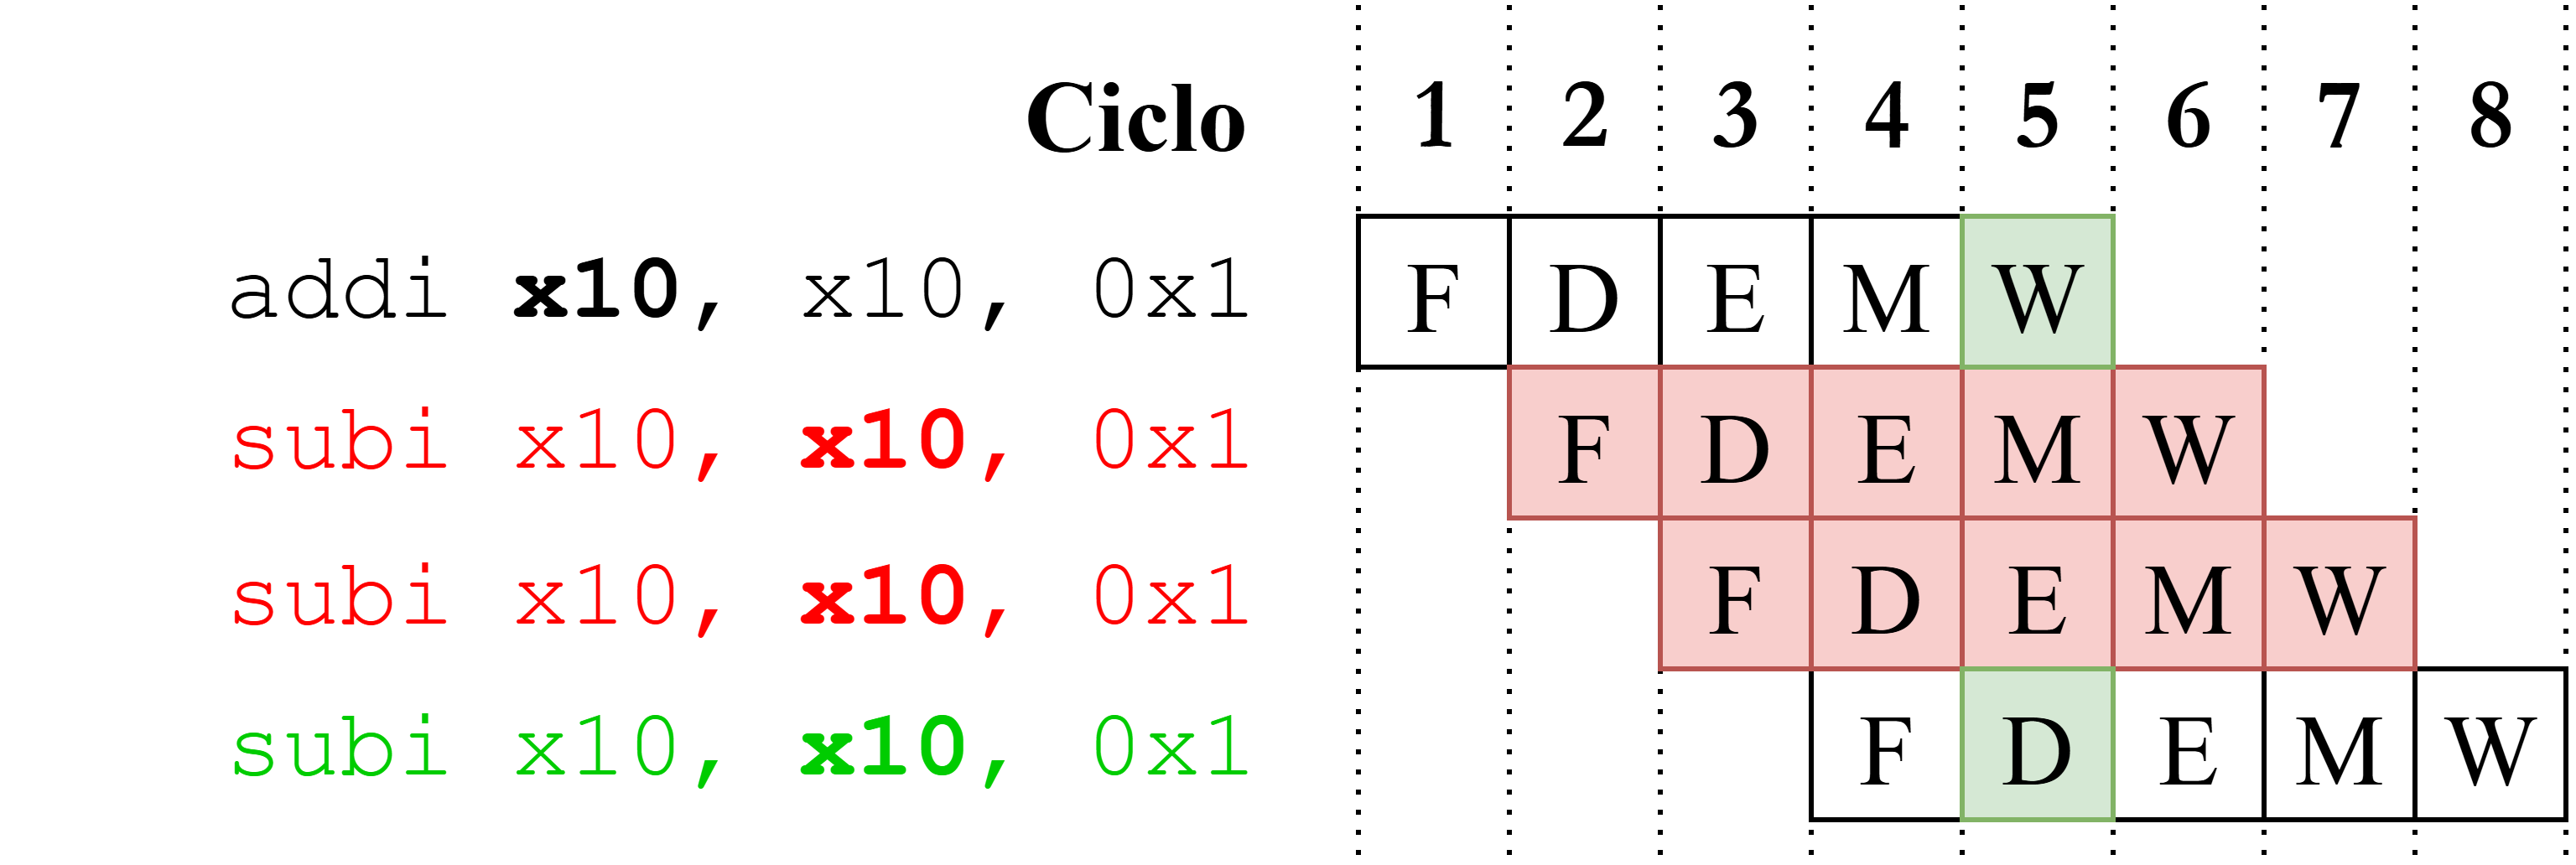
\includegraphics[width=0.53\linewidth]{res/img/diagramas/cap05-03/cap05-03-01-diagrama-dep-raw-ejemplo.png}
  \caption{Ejemplo de una dependencia RAW en una arquitectura segmentada en cinco fases.}
\end{figure}
\vspace{-0.1cm}

La solución (que no sea introducir \textit{nop}s) al problema que supone la ocurrencia de esta clase de escenarios pasa por la aplicación de una técnica denominada \textit{forwarding}. Esta técnica consiste en adelantar el resultado de una instrucción, ya sea aritmético-lógica o una lectura de memoria, directamente a la fase de ejecución de las instrucciones que deban emplear ese dato como operando. En el ejemplo de la Figura 5.13, la instrucción \texttt{subi} podría ejecutar sin problemas justo después del \texttt{addi} si se adelantase el resultado del \texttt{addi} desde la fase de memoria. El forwarding debe hacerse desde la fase de memoria del \texttt{addi} porque 

A continuación, se indicarán las soluciones propuestas al problema de las dependencias de datos del tipo RAW, tanto en el caso de las instrucciones aritmético-lógicas como en el caso de la instrucción de lectura de memoria:

%%%%%%%%%%%%%% Riesgos causados por la sucesión de instrucciones aritmético-lógicas %%%%%%%%%%%%%%%%
\subsubsection{Riesgos causados por la sucesión de instrucciones aritmético-lógicas}

Las señales de la \textit{hazard unit} implicadas en la detección de esta clase de riesgos son:

\begin{itemize}
  \item \textbf{\textit{rs1\_ex}}: la dirección del registro empleado como primer operando de la instrucción, observado en la fase de ejecución.
  \vspace{-0.2cm}
  \item \textbf{\textit{rs2\_ex}}: la dirección del registro empleado como segundo operando de la instrucción, observado en la fase de ejecución.
  \vspace{-0.2cm}
  \item \textbf{\textit{rd\_mem}}: la dirección del registro destino, observado en la fase de acceso a memoria.
  \vspace{-0.2cm}
  \item \textbf{\textit{rd\_wb}}: la dirección del registro destino, observado en la fase de escritura de resultados.
  \vspace{-0.2cm}
  \item \textbf{\textit{rd\_wb}}: la dirección del registro destino, observado en la fase de escritura de resultados.
  \vspace{-0.2cm}
  \item \textbf{\textit{rd\_wb}}: la dirección del registro destino, observado en la fase de escritura de resultados.
\end{itemize}

La \textit{hazard unit} gobierna, además, las señales de selección de dos multiplexores emplazados, cada uno, en una de las entradas de la ALU:

\begin{itemize}
  \item \textbf{\textit{alu\_rs1\_src}}: controla la selección del primer operando de la ALU, que puede ser un dato leído a partir del banco de registros por parte de la instrucción en fase de ejecución, o un resultado adelantado desde la fase de memoria o de \textit{writeback}.
  \vspace{-0.2cm}
  \item \textbf{\textit{alu\_rs2\_src}}: exactamente igual que la anterior, pero aplicada al segundo operando de la ALU.
\end{itemize}

La lógica que rige el proceso de detección de las dependencias por parte de la \textit{hazard unit} es tal y como se indica en la Figura 5.14, siendo el código aplicable tanto en el caso en que la dependencia se diese con el primer registro operando, como si esta se diese con el segundo.

Más allá de lo auto-explicativo del diagrama de flujo que acompaña al código, cabe reseñar el por qué de la condición en la que se evalúa si el registro origen es \texttt{x0} y es que, de darse una dependencia RAW en la que este registro se encontrase involucrado, no tendría sentido realizar un \textit{forwarding} de un registro cuyo valor es constantemente 0, por lo que se evita solventar esta falsa dependencia.

% Figura 5.14: Codigo y pseudo-codigo de la logica empleada en la deteccion y mitigacion de riesgos de datos del tipo RAW en los que esta involucrado el primer registro origen de una instruccion.
\vspace{+0.4cm}
\begin{figure}[h!!!]
\centering
\renewcommand{\arraystretch}{1}

\begin{tabular}{|p{0.95\textwidth}|}
\hline
\textbf{Código}
\\
\hline
\begin{lstlisting}[style=scalaStyleNoNumberingNoBorder2]
io.alu_rs1_src := Mux(
  ((io.rs1_ex === io.rd_mem) & io.reg_wr_enable_mem) & (io.rs1_ex =/= 0.U),
  RsFwSel.ALUResultMemFw,
  Mux(
    ((io.rs1_ex === io.rd_wb) & io.reg_wr_enable_wb) & (io.rs1_ex =/= 0.U),
    RsFwSel.ALUResultWbFw,
    RsFwSel.RegFileData
  )
)
\end{lstlisting}
\\
\hline
\textbf{Diagrama de flujo} \\
\hline

\begin{minipage}{\linewidth}
\centering
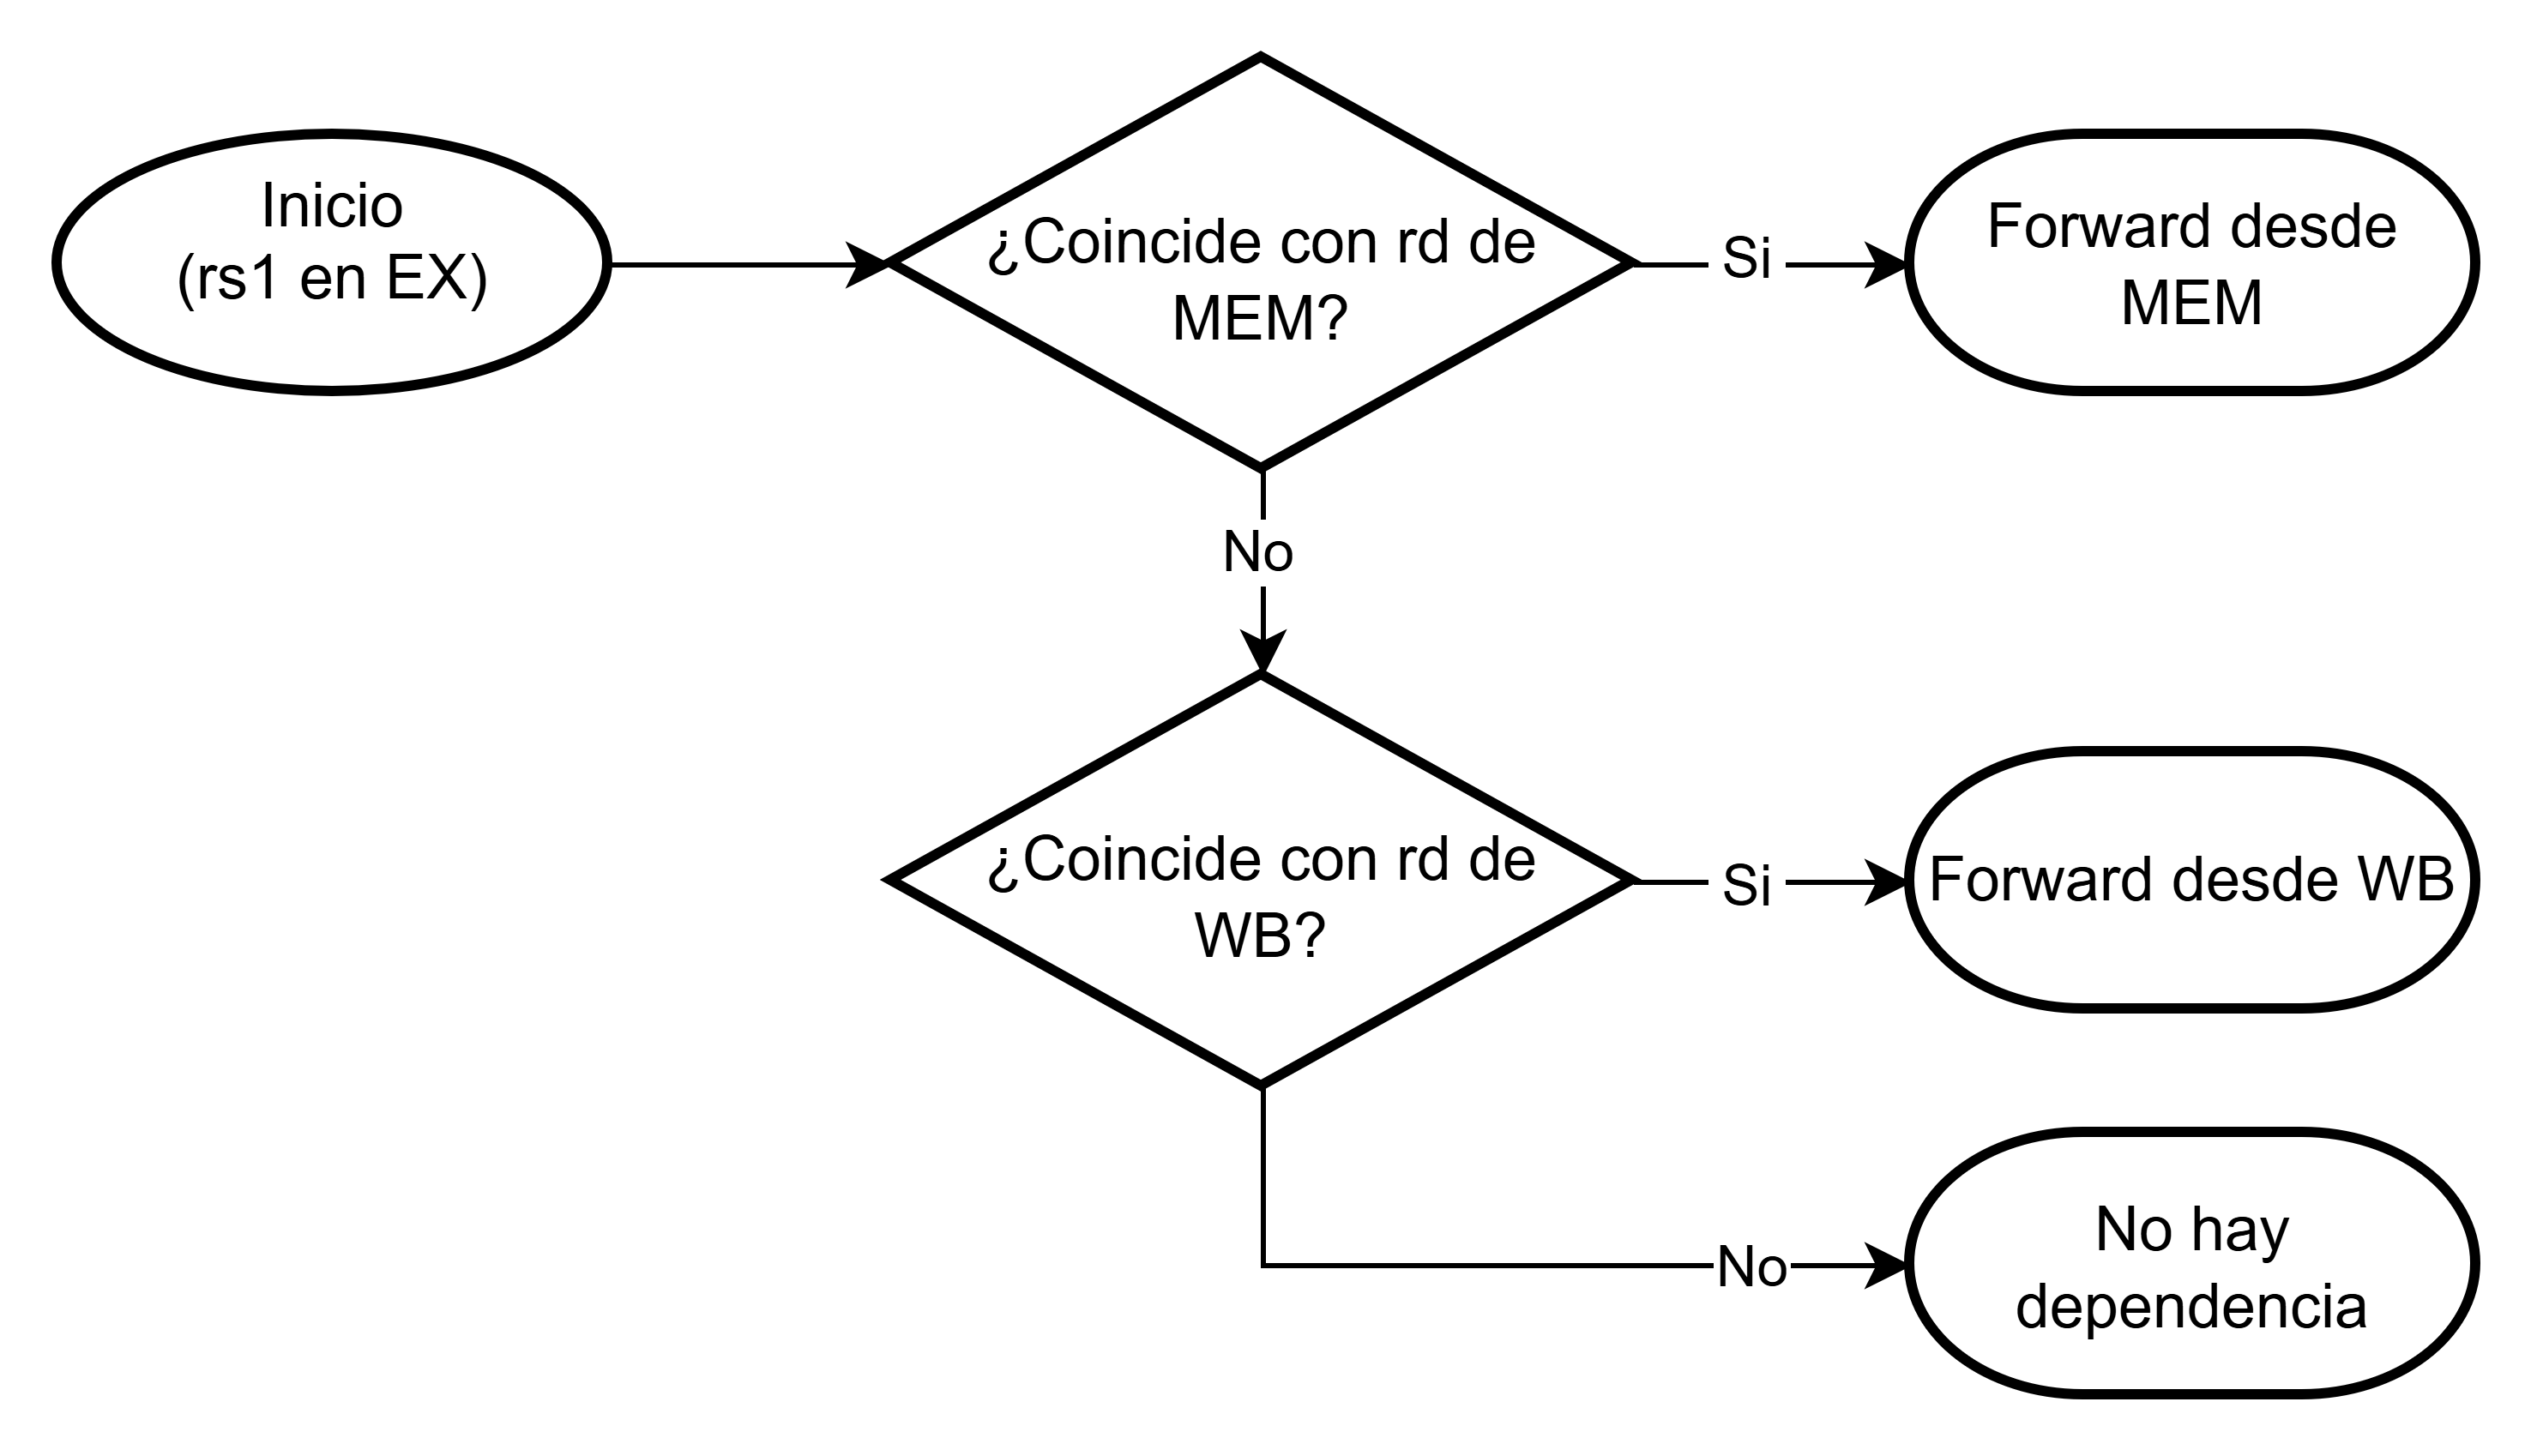
\includegraphics[width=0.65\linewidth]{res/img/diagramas/cap05-03/cap05-03-04-diagrama-flujo-hu.png}
\end{minipage}
\\
\hline
\end{tabular}
\vspace{-0.2cm}
\caption{Implementación en Chisel y diagrama de decisión de la lógica de \textit{forwarding} para la selección del primer operando de la ALU.}
\end{figure}

%%%%%%%%%%%%%% Riesgos en los que se encuentra involucrada la instrucción 'lw' %%%%%%%%%%%%%%%%%%%%%
\subsubsection{Dependencias en las que se encuentra involucrada la instrucción '\texttt{lw}'}

La presencia de la instrucción \texttt{lw} en una dependencia de datos del tipo RAW genera un caso especial que no puede resolverse por medio de la metodología seguida en el apartado anterior. Esto es debido a que el resultado de la instrucción \texttt{lw} no se genera hasta haber completado la lectura de un dato de memoria, lo cual se produce al término de la fase de memoria de la instrucción. En ese momento la instrucción dependiente imediatamente posterior al \texttt{lw} ya habrá completado su fase de ejecución, pero lo habrá hecho con un operando erróneo.

La técnica con la que se resuelve la dependencia consiste en detener el procesamiento de las instrucciones en fases de \textit{fetch} y decodificación cada vez que esta sea detectada. Esto se consigue reteniendo los datos del registro de segmentación que separa las fases de \textit{fetch} y decodificación, y el contador de programa, y haciendo \texttt{flush} del registro de segmentación que separa decodificación y ejecución. Esta retención y limpieza dura tan solo un ciclo, de tal modo que, cuando la instrucción dependiente que no es el \texttt{lw} pase a la fase de ejecución, la \textit{hazard unit} tratará la dependencia como si de cualquier otra dependencia de datos se tratase, adelantando desde el writeback del \textit{lw} a la entrada de la ALU que corresponda, el valor leído de la memoria. Se proporciona en la Figura 5.15 una representación de la resolución del riesgo de datos por medio de esta técnica.

% Figura 5.15: Flujo de ejecucion de dos instrucciones implicadas en una dependencia de datos de tipo RAW, una de las cuales es la instruccion lw.
\vspace{+0.4cm}
\begin{figure}[h]
  \centering
  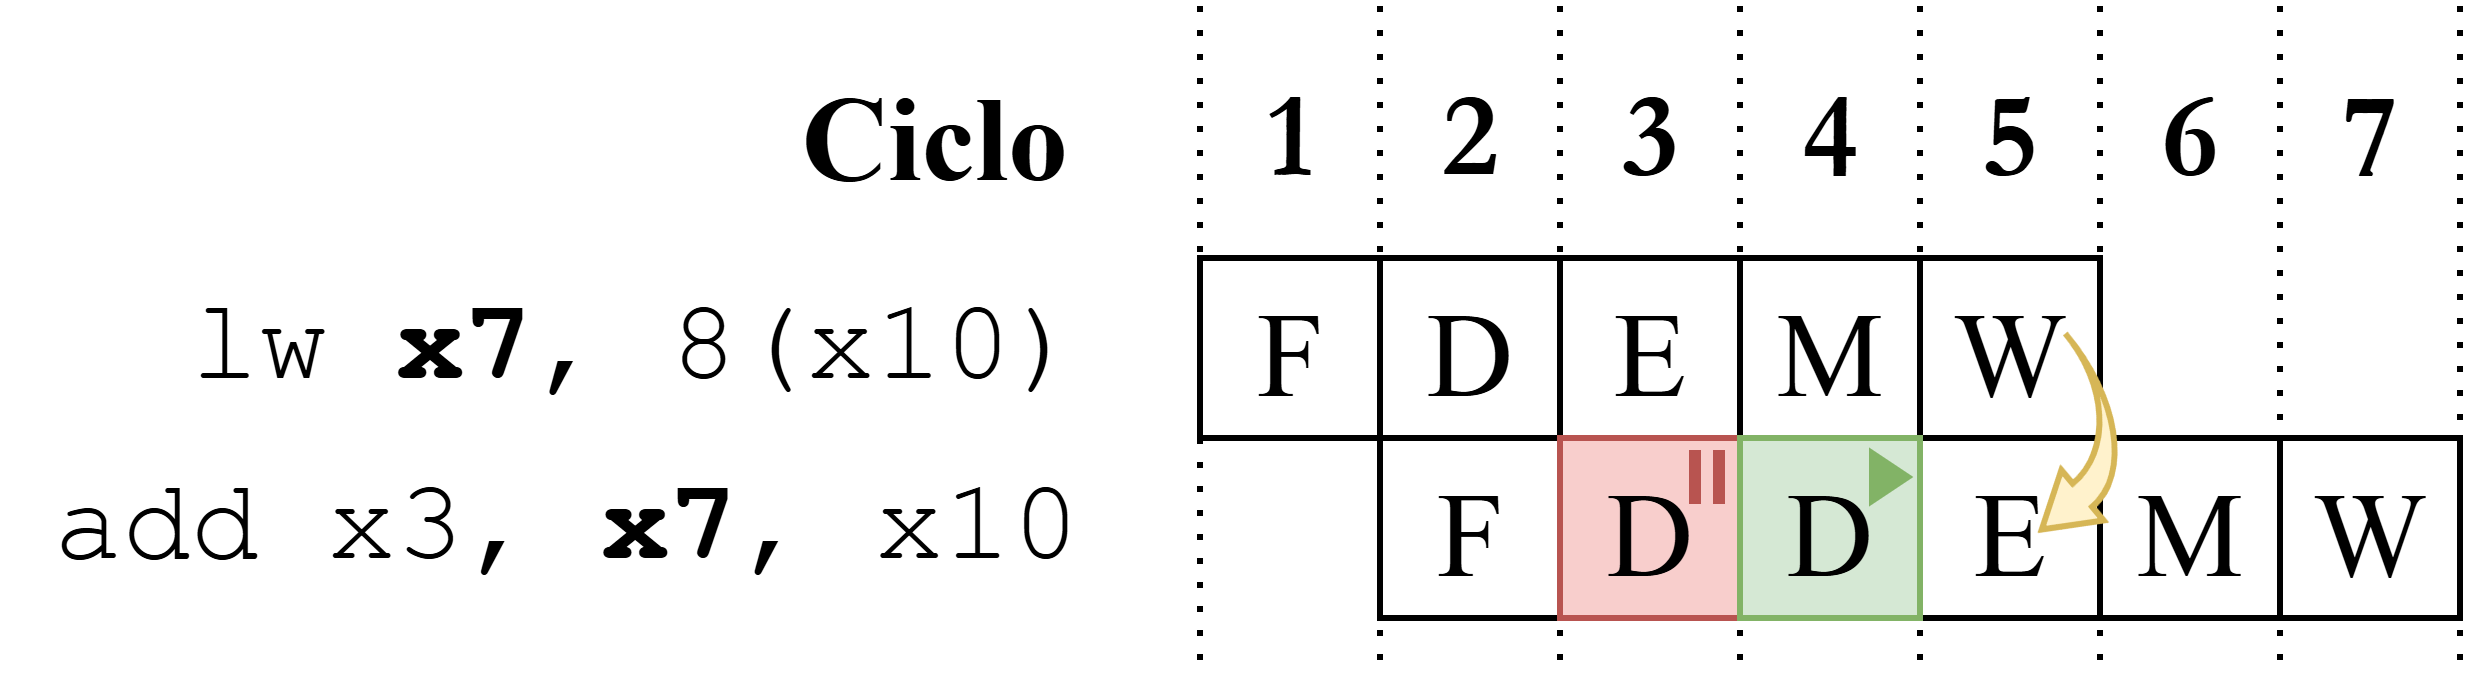
\includegraphics[width=0.6\linewidth]{res/img/diagramas/cap05-03/cap05-03-02-solucion-dep-raw-lw.png}
  \caption{Flujo de ejecución de dos instrucciones implicadas en una dependencia de datos de tipo RAW, una de las cuales es la instrucción \texttt{lw}.}
\end{figure}
\vspace{+0.4cm}

La detención y limpieza de los registros de segmentación mencionados, así como la parada del del contador de programa, se controlan por medio de la señal \texttt{lw\_stall}, cuyo cómputo se realiza según lo indicado en la primera línea del código de la Figura 5.16. La expresión lógica que determina el valor de la señal se compone de las siguientes tres condiciones:

\begin{itemize}
  \item \textbf{C1} $\rightarrow$ \textbf{\texttt{io.ex\_regs\_write\_src(0)}}: en primer lugar, se identifica si una instrucción en fase de ejecución va a provocar la escritura en el banco de registros de un dato leído de memoria. Esto se hace observando el bit menos significativo de la señal \texttt{ex\_regs\_write\_src}, la cual controla la salida del multiplexor en la fase de \textit{writeback} con el que se escoge el dato a escribir en el banco de registros. La salida de este multiplexor podrá ser un resultado calculado en la ALU, la dirección de retorno de un salto o el dato leído en una posición de memoria. En este último caso, el valor del bit menos significativo de la señal \texttt{ex\_regs\_write\_src} es igual a 1.
  
  Que el valor de ese bit sea igual a 1 es condición suficiente y necesaria para asegurar que la instrucción en fase de ejecución es un \texttt{lw}.
  \item \textbf{C2} $\rightarrow$ \textbf{\texttt{io.rs1\_d === io.rd\_ex}}: detección de dependencia de datos RAW entre dos instrucciones consecutivas emplazadas en las fases de decodificación y ejecución. Se observa la dirección del primer registro origen.
  \item \textbf{C2} $\rightarrow$ \textbf{\texttt{io.rs2\_d === io.rd\_ex}}: exactamente igual que la condición anterior, pero observando la dirección del segundo registro origen.
\end{itemize}

En resumen, la expresión lógica con la que se define el valor de la señal \texttt{lw\_stall} es como sigue:

\[
\textit{lw\_stall} = C_1 \land (C_2 \lor C_3)
\]

Si se detecta una dependencia de datos RAW entre instrucciones emplazadas en las fases de decodificación y ejecución ($C_2$ o $C_3$) y, además, se detecta un \texttt{lw} en la fase de ejecución ($C_1$), se detienen el contador de programa y el registro de segmentación \textit{fetch}-decodificación, y se hace \texttt{flush} del registro de segmentación de decodificación-ejecución. De este modo, tan solo el \texttt{lw} podrá avanzar en el pipeline. En el ciclo siguiente a la detección de la dependencia, el \texttt{lw} leerá el dato de memoria, el cual podrá ser adelantado, en el ciclo posterior, a la fase de ejecución de la otra instrucción implicada en la dependencia.

% Figura 5.16: Computo de la señal lw_stall
\vspace{+0.4cm}
\begin{figure}[h!]
\begin{lstlisting}[style=scalaStyle,columns=fullflexible]{}
val lw_stall = io.ex_regs_write_src(0) &
               ((io.rs1_d === io.rd_ex) | (io.rs2_d === io.rd_ex))

io.pc_stall   := lw_stall
io.srFD_stall := lw_stall
io.srDE_flush := lw_stall
\end{lstlisting}
\vspace{-0.4cm}
\caption{Cómputo de la señal \texttt{lw\_stall}.}
\end{figure}

Las señales \texttt{pc\_stall}, \texttt{srFD\_stall} y \texttt{srDE\_flush} controlan, respectivamente, la parada del contador de programa, la detención del registro de segmentación de \textit{fetch}-decodificación, y la limpieza del registro de segmentación de decodificación-ejecución.

Al instanciar el registro de segmentación en el módulo \texttt{CPU}, se indica que la señal de \textit{reset} del registro será la señal \texttt{srDE\_flush} generada por la \textit{hazard unit}, tal y como se observa en el código mostrado en la Figura TODO:

% Figura 5.17: Instanciación, en el módulo CPU, del registro de segmentación que separa las fases de decodificación y ejecución.
\vspace{+0.4cm}
\begin{figure}[h!]
\begin{lstlisting}[style=scalaStyle,columns=fullflexible]{}
val srDE = withReset(hazard_unit.io.srDE_flush){Module(new DE)}
\end{lstlisting}
\vspace{-0.4cm}
\caption{Instanciación, en el módulo \texttt{CPU}, del registro de segmentación que separa las fases de decodificación y ejecución.}
\end{figure}

Por último, se ha adaptado la lógica del módulo \texttt{InstructionFetch} (ver Figura 5.18) de tal modo que el contador de programa avance tan solo cuando el cargador haya indicado que ha terminado su trabajo (valor 1 en el puerto \texttt{instruction\_valid}), y la \textit{hazard unit} lo permita (valor cero en el puerto \texttt{pc\_stall}).

% Figura 5.18: Adaptación del código del módulo InstructionFetch.
\vspace{+0.2cm}
\begin{figure}[h!]
\begin{lstlisting}[style=scalaStyle,columns=fullflexible]{}
when(io.instruction_valid & !io.pc_stall) {
  io.instruction := io.instruction_read_data
  pc := Mux(io.jump_flag_id, io.jump_address_id, pc_plus_four)
} .elsewhen(io.instruction_valid & io.pc_stall) {
  pc             := pc
  io.instruction := io.instruction_read_data
} .otherwise {
  pc             := pc
  io.instruction := 0x00000013.U
}

io.current_pc := pc
io.next_pc    := pc_plus_four
\end{lstlisting}
\vspace{-0.4cm}
\caption{Adaptación del código del módulo InstructionFetch.}
\end{figure}

%%%%%%%%%%%%%%%%%%%%%%%%%%%%%%%%% Resolución de riesgos de control %%%%%%%%%%%%%%%%%%%%%%%%%%%%%%%%%
\subsection{Resolución de riesgos de control}

Una solución sencilla y eficaz al problema generado por los riesgos de control es limpiar el contenido de los registros de segmentación entre las etapas de fetch-decodificación y decodificación-ejecución cada vez que, en la fase de ejecución de una instrucción de salto, se determine que este deba ser tomado. De este modo, tal y como se observa en el ejemplo de la Figura 5.17, todas las instrucciones (máximo 2) que logren introducirse en el pipeline tras la instrucción de salto, no se procesarán completamente y su paso por la arquitectura habrá sido totalmente inocuo.

% Figura 5.17: Diagrama ilustrativo del proceso de mitigación de los riesgos de control.
\vspace{+0.4cm}
\begin{figure}[h]
  \centering
  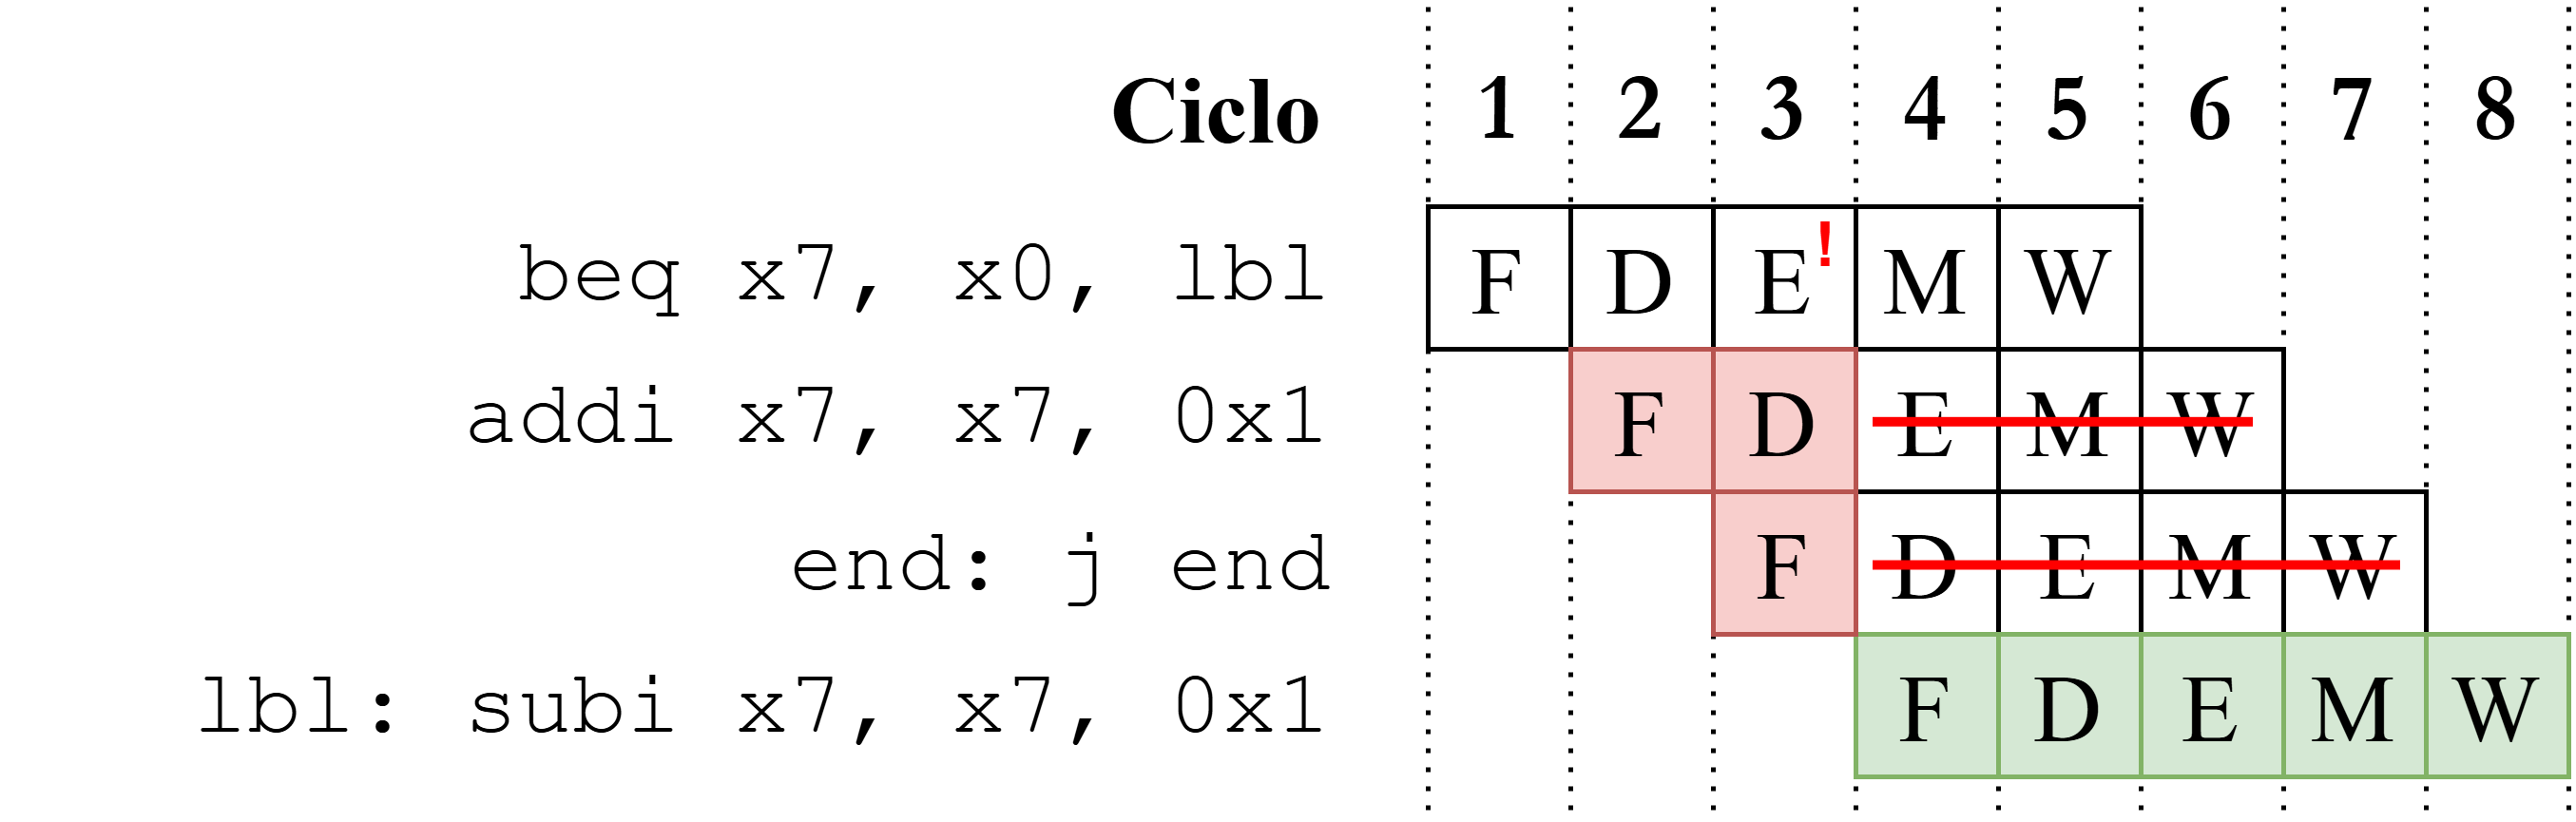
\includegraphics[width=0.6\linewidth]{res/img/diagramas/cap05-03/cap05-03-03-solucion-dep-control.png}
  \caption{Diagrama ilustrativo del proceso de mitigación de los riesgos de control.}
\end{figure}
\vspace{+0.4cm}

Esta solución se implementa por medio del fragmenteo de código de la \textit{hazard unit} mostrado en la Figura 5.18, donde se establece que el valor de la señal de borrado de los registros de segmentación indicados (señales \texttt{srDE\_flush} y \texttt{srFD\_flush}\footnote{La instanciación del registro de segmentación de \textit{fetch}-decodificación en el módulo \texttt{CPU} se lleva a cabo de igual modo que en el caso del registro \texttt{srDE}, indicando que el \textit{reset} del registro será la señal \texttt{srFD\_flush} generada en la \textit{hazard unit}}), será igual al valor del flag de salto observado en la fase de ejecución.

% Figura 5.18: Configuración de la señal de borrado de los registros de segmentación que separan las fases de fetch-decodificación y decodificación-ejecución, conforme al valor del flag de salto en fase de ejecución.
\vspace{+0.4cm}
\begin{figure}[h!]
\begin{lstlisting}[style=scalaStyle,columns=fullflexible]{}
io.srDE_flush := lw_stall | io.ex_jump_flag
io.srFD_flush := io.ex_jump_flag
\end{lstlisting}
\vspace{-0.4cm}
\caption{Configuración de la señal de borrado de los registros de segmentación que separan las fases de fetch-decodificación y decodificación-ejecución, conforme al valor del flag de salto en fase de ejecución.}
\end{figure}
